%% LaTeX Template for ISIT 2020
%%
%% by Stefan M. Moser, October 2017
%% 
%% derived from bare_conf.tex, V1.4a, 2014/09/17, by Michael Shell
%% for use with IEEEtran.cls version 1.8b or later
%%
%% Support sites for IEEEtran.cls:
%%
%% http://www.michaelshell.org/tex/ieeetran/
%% http://moser-isi.ethz.ch/manuals.html#eqlatex
%% http://www.ctan.org/tex-archive/macros/latex/contrib/IEEEtran/
%%

\documentclass[conference,letterpaper]{IEEEtran}

%% depending on your installation, you may wish to adjust the top margin:
\addtolength{\topmargin}{9mm}

%%%%%%
%% Packages:
%% Some useful packages (and compatibility issues with the IEEE format)
%% are pointed out at the very end of this template source file (they are 
%% taken verbatim out of bare_conf.tex by Michael Shell).
%
% *** Do not adjust lengths that control margins, column widths, etc. ***
% *** Do not use packages that alter fonts (such as pslatex).         ***
%
\usepackage[utf8]{inputenc} 
\usepackage[T1]{fontenc}
\usepackage{url}
\usepackage{ifthen}
\usepackage{cite}
\usepackage[cmex10]{amsmath} % Use the [cmex10] option to ensure complicance
                             % with IEEE Xplore (see bare_conf.tex)
\usepackage{amssymb}
\usepackage{amsthm}
\usepackage{graphicx}
\usepackage{mathtools}
\usepackage{bm}
\DeclarePairedDelimiter\abs{\lvert}{\rvert}
\DeclarePairedDelimiter\norm{\lVert}{\rVert}
\DeclarePairedDelimiter\inner{\langle}{\rangle}
\def\P{\mathcal{P}}
\def\E{\mathbb{E}}
\DeclarePairedDelimiter\floor{\lfloor}{\rfloor}
\DeclarePairedDelimiter\ceil{\lceil}{\rceil}
\DeclareMathOperator*{\diag}{diag}
\DeclareMathOperator*{\argmin}{argmin}
%% Please note that the amsthm package must not be loaded with
%% IEEEtran.cls because IEEEtran provides its own versions of
%% theorems. Also note that IEEEXplore does not accepts submissions
%% with hyperlinks, i.e., hyperref cannot be used.

\interdisplaylinepenalty=2500 % As explained in bare_conf.tex


%%%%%%
% correct bad hyphenation here
\hyphenation{op-tical net-works semi-conduc-tor}

% ------------------------------------------------------------
\begin{document}
\title{On the Universally Good Activation Function for One Node Neural Network} 

% %%% Single author, or several authors with same affiliation:
% \author{%
%   \IEEEauthorblockN{Stefan M.~Moser}
%   \IEEEauthorblockA{ETH Zürich\\
%                     ISI (D-ITET)\\
%                     CH-8092 Zürich, Switzerland\\
%                     Email: moser@isi.ee.ethz.ch}
% }


%%% Several authors with up to three affiliations:
\author{%
  \IEEEauthorblockN{Shao-Lun Huang}
  \IEEEauthorblockA{ETH Zürich\\
                    ISI (D-ITET), ETH Zentrum\\
                    CH-8092 Zürich, Switzerland\\
                    Email: moser@isi.ee.ethz.ch}
  \and
  \IEEEauthorblockN{Feng Zhao}
  \IEEEauthorblockA{Hogwarts School of Witchcraft and Wizardry\\
                    Hogwarts Castle\\ 
                    1714 Hogsmeade, Scotland\\
                    Email: \{dumbledore, potter\}@hogwarts.edu}
}


%%% Many authors with many affiliations:
% \author{%
%   \IEEEauthorblockN{Albus Dumbledore\IEEEauthorrefmark{1},
%                     Olympe Maxime\IEEEauthorrefmark{2},
%                     Stefan M.~Moser\IEEEauthorrefmark{3}\IEEEauthorrefmark{4},
%                     and Harry Potter\IEEEauthorrefmark{1}}
%   \IEEEauthorblockA{\IEEEauthorrefmark{1}%
%                     Hogwarts School of Witchcraft and Wizardry,
%                     1714 Hogsmeade, Scotland,
%                     \{dumbledore, potter\}@hogwarts.edu}
%   \IEEEauthorblockA{\IEEEauthorrefmark{2}%
%                     Beauxbatons Academy of Magic,
%                     1290 Pyrénées, France,
%                     maxime@beauxbatons.edu}
%   \IEEEauthorblockA{\IEEEauthorrefmark{3}%
%                     ETH Zürich, ISI (D-ITET), ETH Zentrum, 
%                     CH-8092 Zürich, Switzerland,
%                     moser@isi.ee.ethz.ch}
%   \IEEEauthorblockA{\IEEEauthorrefmark{4}%
%                     National Chiao Tung University (NCTU), 
%                     Hsinchu, Taiwan,
%                     moser@isi.ee.ethz.ch}
% }


\maketitle

%%%%%%
%% Abstract: 
%% If your paper is eligible for the student paper award, please add
%% the comment "THIS PAPER IS ELIGIBLE FOR THE STUDENT PAPER
%% AWARD." as a first line in the abstract. 
%% For the final version of the accepted paper, please do not forget
%% to remove this comment!
%%
\begin{abstract}
Non-linear activation function plays vital role in artificial neural network.
In this paper, we show that under certain conditions Hermite orthogonal polynomial
is universally good for orthogonal input features. Our study shares insight in the expressive
power of neural network and can guide the choice of activation function in practice.
\end{abstract}


%% The paper must be self-contained. However, if you are referring to
%% a full version for checking certain proofs, please provide the
%% publically accessible location below.  If the paper is completely
%% self-contained, you can remove the following line from your
%% submission.
\textit{A full version of this paper is accessible at:}
\url{https://2020.ieee-isit.org/} 

\section{Introduction}
In artificial neural network, activation functions are applied to linear combinations of input features from last layer and contribute magically to the whole system. There are many choices for activation function \cite{laudani2015training} and none of them performs best for all problems. Previous study of activation function focuses mostly on the training efficiency and cost when choosing activation function. However, theoretical property is also important as a gurantee to the functionality of activation function in neural network. In this paper, we study how the activation function influences the network loss when the activation term is contrained to a small perturbation of linear function.

Besides local perturbation assumption, we consider the simplest neural network with one output node and several input node. We also require the input features are orthogonal to each other. This can be simply achieved by commonly used techniques such as PCA. Our measure of activation function is not restricted to one specific problem but is averaged over many different problems. We find that the averaged loss function is minimized when the perturbation term is Hermite orthogonal polynomial. Hermite polynomial as activation function has been argued beneficial previously \cite{ma2005constructive} and our result confirms this fact to some extent.

The paper is organized as follows: In Section \ref{sec:mm}, the universally good activation function problem
is formulated mathematically. In Section \ref{sec:hp}, the Hermite polynomial solution for our problem is briefly deducted. In Section \ref{sec:er}, numerical experiments are conducted to verify our results.
In Section \ref{sec:con}, conclusion is given.

Throught this paper, we use $X$ to represent random variables, $\underline{X}$ to represent random vectors, $\bm{X}$ to represent random matrix,
lower case $x$ to represent a numerical value, $\underline{x}$ as a numerical vector and $\bm{x}$ as numerical matrix.

\section{Mathematical Model}\label{sec:mm}
We consider one node neural networks, whose structure is shown in Figure \ref{fig:ns}.
Given a k dimensional random vector $\underline{X}=(X_1, \dots, X_k)$ and a random variable $Y$. Our goal is to predict $Y$ using the neural network with $\underline{X}$ as input. To be more specific,
$Y$ is approximated by $ \sigma(\sum_{i=1}^k w_i X_i)$. For a given problem, we have $n$ data pairs $(x_1, y_1), \dots, (x_n, y_n)$ and the L2 loss function is given by
$\ell_2(\underline{y}, \bm{x}) = \norm{\underline{y} - \sigma(\sum_{i=1}^k w_i \underline{x}_i)}^2 $ where $\underline{x}_i= (x_{i1}, \dots, x_{in})^T$ is the i-th column of the feature vector $\bm{x}$ and
$\underline{y} = (y_1, \dots, y_n)$ is the label vector. $\sigma$ is applied to a vector elementwise.
The optimal weight for a given activation function $\sigma$ is the solution to $\min \ell_2(\underline{y}, \bm{x})$.
\begin{figure}\label{fig:ns}
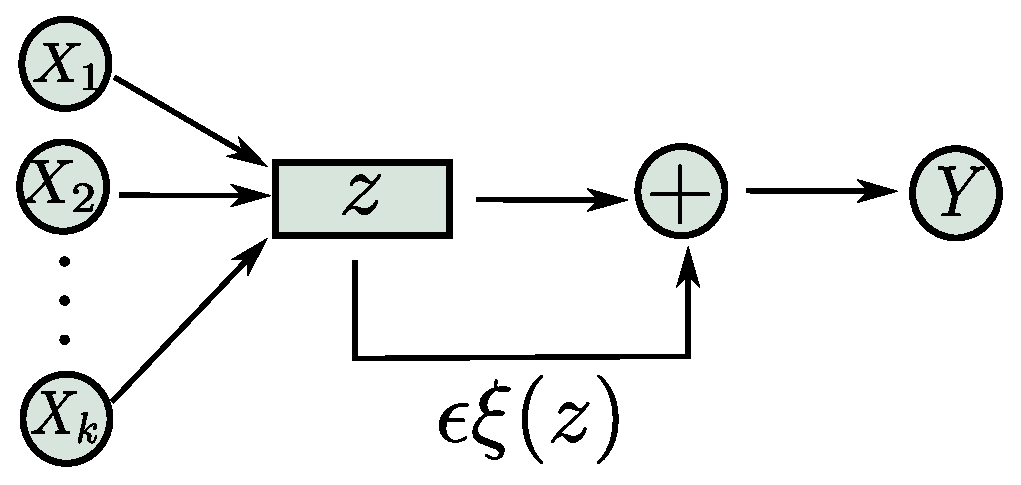
\includegraphics[width=\linewidth]{network_structure.eps}
\end{figure}

For different problems, we suppose $\underline{y}, \bm{x}$ are drawing from some distribution $G$. That is, we treat them as random vectors and rewrite them as $\underline{Y}, \bm{X}$ and we are insterested to find a function $\sigma$ which minimizes
$\E[ \min \ell_2(\underline{Y}, \bm{X})]$. Since $w_i$ is determined by $\underline{y}, \bm{x}$, it can also be converted to random variable $W_i$.
Our contraint on the activation function $\sigma$ is that
$\sigma(z) = z + \epsilon \xi(z)$.
$\epsilon$ is a small constant.
$\E[\xi(\bm{X}\underline{W})]=1$ where $\bm{X}\underline{W} = \sum_{i=1}^k W_i \underline{X}_i$ and  $\underline{W}=(W_1, \dots, W_k)$.


\section{Hermite Polynomials}\label{sec:hp}

Accepted papers will be published in full. 
A program booklet and a book of abstracts will also be
distributed at the Symposium to serve as a guide to the sessions.

The deadline for the submission of the final camera-ready paper will
be announced in due course.  Accepted papers not submitted by that
date will not appear in the ISIT proceedings and will not be included
in the technical program of the ISIT.


\section{Experiment Result}\label{sec:er}

\subsection{Templates}

The paper (A4 or letter size, double-column format, not exceeding
5~pages) should be formatted as shown in this sample \LaTeX{} file
\cite{Laport:LaTeX, GMS:LaTeXComp, oetiker_latex, typesetmoser}.

The use of Microsoft Word instead of \LaTeX{} is strongly
discouraged. However, acceptable formatting may be achieved by using
the template that can be downloaded from the ISIT 2020 website:
\begin{center}
  \url{https://2020.ieee-isit.org/}
\end{center}

Users of other text processing systems should attempt to duplicate the
style of this example, in particular the sizes and type of font, as
closely as possible.


\subsection{Formatting}

The style of references, equations, figures, tables, etc., should be
the same as for the \emph{IEEE Transactions on Information
  Theory}. The source file of this template paper contains many more
instructions on how to format your paper. So, example code for
different numbers of authors, for figures and tables, and references
can be found (they are commented out).

%%%%%%
%% An example of a floating figure using the graphicx package.
%% Note that \label must occur AFTER (or within) \caption.
%% For figures, \caption should occur after the \includegraphics.
%%
% \begin{figure}[htbp]
%   \centering
%   \includegraphics[width=0.3\textwidth]{myfigure}
%   % where an .eps filename suffix will be assumed under latex,
%   % and a .pdf suffix will be assumed for pdflatex
%   \caption{Simulation results.}
%   \label{fig:sim}
% \end{figure}
%%%%%%

%%%%%%
%% An example of a double column floating figure using two subfigures.
%% (The subfigure.sty package must be loaded for this to work.)  The
%% subfigure \label commands are set within each subfigure command,
%% the \label for the overall figure must come after \caption.  
%% \hfil must be used as a separator to get equal spacing
%%
% \begin{figure*}[htbp]
%   \centerline{\subfigure[Case I]{\includegraphics[width=2.5in]{subfigcase1}
%       % where an .eps filename suffix will be assumed under latex,
%       % and a .pdf suffix will be assumed for pdflatex
%       \label{fig:first_case}}
%     \hfil
%     \subfigure[Case II]{\includegraphics[width=2.5in]{subfigcase2}
%       % where an .eps filename suffix will be assumed under latex,
%       % and a .pdf suffix will be assumed for pdflatex
%       \label{fig:second_case}}}
%   \caption{Simulation results.}
%   \label{fig:sim}
% \end{figure*}
%%%%%%

%%%%%%
%% An example of a floating table. 
%% Note that, for IEEE style tables, the \caption command should come
%% BEFORE the table. Table text will default to \footnotesize as IEEE
%% normally uses this smaller font for tables.  The \label must come
%% after \caption as always.
%%
% \begin{table}[htbp]
%   % increase table row spacing, adjust to taste
%   \renewcommand{\arraystretch}{1.3}
%   \caption{An Example of a Table}
%   \label{tab:table_example}
%   \centering
%   % Some packages, such as MDW tools, offer better commands for making tables
%   % than the plain LaTeX2e tabular which is used here.
%   \begin{tabular}{|c||c|}
%     \hline
%     One & Two\\
%     \hline
%     Three & Four\\
%     \hline
%   \end{tabular}
% \end{table}
%%%%%%


For instructions on how to typeset math, in particular for equation
arrays with broken equations, we refer to \cite{typesetmoser}.

Pages should not be numbered and there should be no footer or header
(both will be added during the production of the proceedings). The
affiliation shown for authors should constitute a sufficient mailing
address for persons who wish to write for more details about the
paper.


\subsection{PDF Requirements}

Only electronic submissions in form of a PDF file will be
accepted. The PDF file has to be PDF/A compliant. A common problem is
missing fonts. Make sure that all fonts are embedded. (In some cases,
printing a PDF to a PostScript file, and then creating a new PDF with
Acrobat Distiller, may do the trick.) More information (including
suitable Acrobat Distiller Settings) is available from the IEEE
website \cite{IEEE:pdfsettings, IEEE:AuthorToolbox}.


\section{Conclusion}\label{sec:con}

We conclude by pointing out that on the last page the columns need to
balanced. Instructions for that purpose are given in the source file.

Moreover, example code for an appendix (or appendices) can also be
found in the source file (they are commented out).

%%%%%%
%% Appendix:
%% If needed a single appendix is created by
%%
%\appendix
%%
%% If several appendices are needed, then the command
%%
% \appendices
%%
%% in combination with further \section-commands can be used.
%%%%%%


\section*{Acknowledgment}

We are indebted to Michael Shell for maintaining and improving
\texttt{IEEEtran.cls}. 


%%%%%%
%% To balance the columns at the last page of the paper use this
%% command:
%%
%\enlargethispage{-1.2cm} 
%%
%% If the balancing should occur in the middle of the references, use
%% the following trigger:
%%
\IEEEtriggeratref{3}
%%
%% which triggers a \newpage (i.e., new column) just before the given
%% reference number. Note that you need to adapt this if you modify
%% the paper.  The "triggered" command can be changed if desired:
%%
%\IEEEtriggercmd{\enlargethispage{-20cm}}
%%
%%%%%%


%%%%%%
%% References:
%% We recommend the usage of BibTeX:
%%
%\bibliographystyle{IEEEtran}
%\bibliography{definitions,bibliofile}
%%
%% where we here have assume the existence of the files
%% definitions.bib and bibliofile.bib.
%% BibTeX documentation can be obtained at:
%% http://www.ctan.org/tex-archive/biblio/bibtex/contrib/doc/
%%%%%%


%% Or you use manual references (pay attention to consistency and the
%% formatting style!):
\bibliographystyle{plain}
\bibliography{exportlist}


\end{document}


%%%%%%
%% Some comments about useful packages
%% (extract from bare_conf.tex by Michael Shell)
%%

% *** MISC UTILITY PACKAGES ***
%
%\usepackage{ifpdf}
% Heiko Oberdiek's ifpdf.sty is very useful if you need conditional
% compilation based on whether the output is pdf or dvi.
% usage:
% \ifpdf
%   % pdf code
% \else
%   % dvi code
% \fi
% The latest version of ifpdf.sty can be obtained from:
% http://www.ctan.org/pkg/ifpdf
% Also, note that IEEEtran.cls V1.7 and later provides a builtin
% \ifCLASSINFOpdf conditional that works the same way.
% When switching from latex to pdflatex and vice-versa, the compiler may
% have to be run twice to clear warning/error messages.


% *** CITATION PACKAGES ***
%
%\usepackage{cite}
% cite.sty was written by Donald Arseneau
% V1.6 and later of IEEEtran pre-defines the format of the cite.sty package
% \cite{} output to follow that of the IEEE. Loading the cite package will
% result in citation numbers being automatically sorted and properly
% "compressed/ranged". e.g., [1], [9], [2], [7], [5], [6] without using
% cite.sty will become [1], [2], [5]--[7], [9] using cite.sty. cite.sty's
% \cite will automatically add leading space, if needed. Use cite.sty's
% noadjust option (cite.sty V3.8 and later) if you want to turn this off
% such as if a citation ever needs to be enclosed in parenthesis.
% cite.sty is already installed on most LaTeX systems. Be sure and use
% version 5.0 (2009-03-20) and later if using hyperref.sty.
% The latest version can be obtained at:
% http://www.ctan.org/pkg/cite
% The documentation is contained in the cite.sty file itself.


% *** GRAPHICS RELATED PACKAGES ***
%
\ifCLASSINFOpdf
  % \usepackage[pdftex]{graphicx}
  % declare the path(s) where your graphic files are
  % \graphicspath{{../pdf/}{../jpeg/}}
  % and their extensions so you won't have to specify these with
  % every instance of \includegraphics
  % \DeclareGraphicsExtensions{.pdf,.jpeg,.png}
\else
  % or other class option (dvipsone, dvipdf, if not using dvips). graphicx
  % will default to the driver specified in the system graphics.cfg if no
  % driver is specified.
  % \usepackage[dvips]{graphicx}
  % declare the path(s) where your graphic files are
  % \graphicspath{{../eps/}}
  % and their extensions so you won't have to specify these with
  % every instance of \includegraphics
  % \DeclareGraphicsExtensions{.eps}
\fi
% graphicx was written by David Carlisle and Sebastian Rahtz. It is
% required if you want graphics, photos, etc. graphicx.sty is already
% installed on most LaTeX systems. The latest version and documentation
% can be obtained at: 
% http://www.ctan.org/pkg/graphicx
% Another good source of documentation is "Using Imported Graphics in
% LaTeX2e" by Keith Reckdahl which can be found at:
% http://www.ctan.org/pkg/epslatex
%
% latex, and pdflatex in dvi mode, support graphics in encapsulated
% postscript (.eps) format. pdflatex in pdf mode supports graphics
% in .pdf, .jpeg, .png and .mps (metapost) formats. Users should ensure
% that all non-photo figures use a vector format (.eps, .pdf, .mps) and
% not a bitmapped formats (.jpeg, .png). The IEEE frowns on bitmapped formats
% which can result in "jaggedy"/blurry rendering of lines and letters as
% well as large increases in file sizes.
%
% You can find documentation about the pdfTeX application at:
% http://www.tug.org/applications/pdftex


% *** MATH PACKAGES ***
%
%\usepackage{amsmath}
% A popular package from the American Mathematical Society that provides
% many useful and powerful commands for dealing with mathematics.
%
% Note that the amsmath package sets \interdisplaylinepenalty to 10000
% thus preventing page breaks from occurring within multiline equations. Use:
%\interdisplaylinepenalty=2500
% after loading amsmath to restore such page breaks as IEEEtran.cls normally
% does. amsmath.sty is already installed on most LaTeX systems. The latest
% version and documentation can be obtained at:
% http://www.ctan.org/pkg/amsmath


% *** SPECIALIZED LIST PACKAGES ***
%
%\usepackage{algorithmic}
% algorithmic.sty was written by Peter Williams and Rogerio Brito.
% This package provides an algorithmic environment fo describing algorithms.
% You can use the algorithmic environment in-text or within a figure
% environment to provide for a floating algorithm. Do NOT use the algorithm
% floating environment provided by algorithm.sty (by the same authors) or
% algorithm2e.sty (by Christophe Fiorio) as the IEEE does not use dedicated
% algorithm float types and packages that provide these will not provide
% correct IEEE style captions. The latest version and documentation of
% algorithmic.sty can be obtained at:
% http://www.ctan.org/pkg/algorithms
% Also of interest may be the (relatively newer and more customizable)
% algorithmicx.sty package by Szasz Janos:
% http://www.ctan.org/pkg/algorithmicx


% *** ALIGNMENT PACKAGES ***
%
%\usepackage{array}
% Frank Mittelbach's and David Carlisle's array.sty patches and improves
% the standard LaTeX2e array and tabular environments to provide better
% appearance and additional user controls. As the default LaTeX2e table
% generation code is lacking to the point of almost being broken with
% respect to the quality of the end results, all users are strongly
% advised to use an enhanced (at the very least that provided by array.sty)
% set of table tools. array.sty is already installed on most systems. The
% latest version and documentation can be obtained at:
% http://www.ctan.org/pkg/array

% IEEEtran contains the IEEEeqnarray family of commands that can be used to
% generate multiline equations as well as matrices, tables, etc., of high
% quality.


% *** SUBFIGURE PACKAGES ***
%\ifCLASSOPTIONcompsoc
%  \usepackage[caption=false,font=normalsize,labelfont=sf,textfont=sf]{subfig}
%\else
%  \usepackage[caption=false,font=footnotesize]{subfig}
%\fi
% subfig.sty, written by Steven Douglas Cochran, is the modern replacement
% for subfigure.sty, the latter of which is no longer maintained and is
% incompatible with some LaTeX packages including fixltx2e. However,
% subfig.sty requires and automatically loads Axel Sommerfeldt's caption.sty
% which will override IEEEtran.cls' handling of captions and this will result
% in non-IEEE style figure/table captions. To prevent this problem, be sure
% and invoke subfig.sty's "caption=false" package option (available since
% subfig.sty version 1.3, 2005/06/28) as this is will preserve IEEEtran.cls
% handling of captions.
% Note that the Computer Society format requires a larger sans serif font
% than the serif footnote size font used in traditional IEEE formatting
% and thus the need to invoke different subfig.sty package options depending
% on whether compsoc mode has been enabled.
%
% The latest version and documentation of subfig.sty can be obtained at:
% http://www.ctan.org/pkg/subfig


% *** FLOAT PACKAGES ***
%
%\usepackage{fixltx2e}
% fixltx2e, the successor to the earlier fix2col.sty, was written by
% Frank Mittelbach and David Carlisle. This package corrects a few problems
% in the LaTeX2e kernel, the most notable of which is that in current
% LaTeX2e releases, the ordering of single and double column floats is not
% guaranteed to be preserved. Thus, an unpatched LaTeX2e can allow a
% single column figure to be placed prior to an earlier double column
% figure.
% Be aware that LaTeX2e kernels dated 2015 and later have fixltx2e.sty's
% corrections already built into the system in which case a warning will
% be issued if an attempt is made to load fixltx2e.sty as it is no longer
% needed.
% The latest version and documentation can be found at:
% http://www.ctan.org/pkg/fixltx2e


%\usepackage{stfloats}
% stfloats.sty was written by Sigitas Tolusis. This package gives LaTeX2e
% the ability to do double column floats at the bottom of the page as well
% as the top. (e.g., "\begin{figure*}[!b]" is not normally possible in
% LaTeX2e). It also provides a command:
%\fnbelowfloat
% to enable the placement of footnotes below bottom floats (the standard
% LaTeX2e kernel puts them above bottom floats). This is an invasive package
% which rewrites many portions of the LaTeX2e float routines. It may not work
% with other packages that modify the LaTeX2e float routines. The latest
% version and documentation can be obtained at:
% http://www.ctan.org/pkg/stfloats
% Do not use the stfloats baselinefloat ability as the IEEE does not allow
% \baselineskip to stretch. Authors submitting work to the IEEE should note
% that the IEEE rarely uses double column equations and that authors should try
% to avoid such use. Do not be tempted to use the cuted.sty or midfloat.sty
% packages (also by Sigitas Tolusis) as the IEEE does not format its papers in
% such ways.
% Do not attempt to use stfloats with fixltx2e as they are incompatible.
% Instead, use Morten Hogholm'a dblfloatfix which combines the features
% of both fixltx2e and stfloats:
%
% \usepackage{dblfloatfix}
% The latest version can be found at:
% http://www.ctan.org/pkg/dblfloatfix


% *** PDF and URL PACKAGES ***
%
%\usepackage{url}
% url.sty was written by Donald Arseneau. It provides better support for
% handling and breaking URLs. url.sty is already installed on most LaTeX
% systems. The latest version and documentation can be obtained at:
% http://www.ctan.org/pkg/url
% Basically, \url{my_url_here}.



% *** Do not adjust lengths that control margins, column widths, etc. ***
% *** Do not use packages that alter fonts (such as pslatex).         ***
%%%%%%


%%% Local Variables:
%%% mode: latex
%%% TeX-master: t
%%% End:
